\documentclass{article}
\usepackage[submission]{../colm2026_conference}
\usepackage[utf8]{inputenc}
\usepackage[T1]{fontenc}
\usepackage{microtype}
\usepackage{hyperref}
\usepackage{url}
\usepackage{booktabs}
\usepackage{longtable}
\usepackage{array}
\usepackage{graphicx}
\usepackage{amsmath,amssymb}
\usepackage{caption}
\usepackage{lineno}

\definecolor{darkblue}{rgb}{0, 0, 0.5}
\hypersetup{
  colorlinks=true,
  citecolor=darkblue,
  linkcolor=darkblue,
  urlcolor=darkblue,
  pdfauthor={Anonymous},
  pdftitle={Channel Sets Drift During Long Reasoning},
  pdfsubject={COLM 2026 submission},
  pdfkeywords={},
  pdfcreator={LaTeX},
  pdfproducer={}
}
\urlstyle{same}
\graphicspath{{figures/}}
\setkeys{Gin}{width=0.92\linewidth,height=0.27\textheight,keepaspectratio}
\setcounter{secnumdepth}{2}
\newcommand{\tightlist}{\setlength{\itemsep}{0pt}\setlength{\parskip}{0pt}}

\title{Channel Sets Drift During Long Reasoning\\\large A Measurement Regime For Static W4A16 Protection}
\author{Anonymous Authors}

\begin{document}
\ifcolmsubmission
\linenumbers
\fi
\maketitle

\begin{abstract}
W4A16 long-reasoning quantization often protects a fixed set of
high-risk activation channels. Channel-Set asks whether that static unit
is stable enough to support a positive method. The current evidence
supports a measurement/regime result rather than a confirmed adaptive
method: top-1\% strict set-leaving is \(0.566235\) for
Granite-Small, \(0.533713\) for Nemotron-3, \(0.670573\) for
DeepSeek-R1-Distill, and \(0.673611\) for Falcon-H1. This
measurement tensions a competing account: OSC-style static protection is
motivated by token-persistent outlier channel clusters, but long-decode
high-risk sets drift at the trace level. the adaptive clip candidate
remains parked because the cached gate path was contaminated and the
fresh three-model same-row ParoQuant-vs-tight-clip matrix is missing.
The paper contributes a scoped regime claim: static channel-set
protection is a weak abstraction for these long-reasoning traces, and
any future positive method must beat ParoQuant/static baselines under
split-clean same-row native evidence.
\end{abstract}

\hypertarget{claim-boundary-box}{%
\subsection{Claim-Boundary Box}\label{claim-boundary-box}}

\begingroup\small
\begin{longtable}[]{@{}lll@{}}
\toprule
\begin{minipage}[b]{0.30\columnwidth}\raggedright
Supported\strut
\end{minipage} & \begin{minipage}[b]{0.30\columnwidth}\raggedright
Unsupported\strut
\end{minipage} & \begin{minipage}[b]{0.30\columnwidth}\raggedright
Future-only\strut
\end{minipage}\tabularnewline
\midrule
\endhead
\begin{minipage}[t]{0.30\columnwidth}\raggedright
Top-1\% strict set-leaving is high across Granite-Small, Nemotron-3,
DeepSeek-R1-Distill, and Falcon-H1: \(0.533713\) to
\(0.673611\).\strut
\end{minipage} & \begin{minipage}[t]{0.30\columnwidth}\raggedright
A confirmed-positive claim is unsupported.\strut
\end{minipage} & \begin{minipage}[t]{0.30\columnwidth}\raggedright
the adaptive clip candidate can become a positive only after fresh
split-clean native paired materialization.\strut
\end{minipage}\tabularnewline
\begin{minipage}[t]{0.30\columnwidth}\raggedright
Drift is not a single-threshold artifact for the models with
threshold-sweep artifacts.\strut
\end{minipage} & \begin{minipage}[t]{0.30\columnwidth}\raggedright
the adaptive clip candidate is not confirmed and does not beat ParoQuant
in a claim-ready way.\strut
\end{minipage} & \begin{minipage}[t]{0.30\columnwidth}\raggedright
A GPU/native systems card remains separate from this paper-finalization
pass.\strut
\end{minipage}\tabularnewline
\begin{minipage}[t]{0.30\columnwidth}\raggedright
the router audit, the clean-denominator audit, and the defense-bundle
audit blockers are real schema/floor/native-pairing blockers.\strut
\end{minipage} & \begin{minipage}[t]{0.30\columnwidth}\raggedright
No held-out method confirmation is claimed.\strut
\end{minipage} & \begin{minipage}[t]{0.30\columnwidth}\raggedright
OSC/DecDEC defenses can validate a future method after same-row pairing
exists.\strut
\end{minipage}\tabularnewline
\bottomrule
\end{longtable}
\endgroup

\hypertarget{introduction}{%
\subsection{1. Introduction}\label{introduction}}

Long reasoning changes which activation channels matter. A static W4A16
outlier-protection method can work only if the protected channel set
remains stable enough across the reasoning trace. The Channel-Set
campaign tested adaptive possibilities, but the confirmed result is
simpler and sharper: the set itself moves.

This measurement tensions a competing account. Recent W4A16 work such as
OSC \citep{osc2026} motivates static protection by arguing activation
outliers form token-persistent channel clusters, a fixed object stable
enough to protect once. Our long-decode measurement shows the opposite
for the top-1\% high-risk set: \(53\)-\(67\)\% of later
high-risk channels lie outside the set selected early in the trace. The
two are reconcilable: token-local clusters can persist while the
trace-level high-risk set drifts. That reconciliation is the point.
Static protection chosen from an early window is the wrong granularity
for long reasoning, and any method inheriting it must be validated
against trace-level drift, not token-local persistence alone.

This matters for both method design and evaluation. If later high-risk
channels leave the early protected set, then a static top-channel
abstraction is incomplete. If an adaptive method appears to win without
a paired ParoQuant/static baseline on the same rows, the win may be a
cache artifact or a contaminated split artifact rather than a real
method.

Contributions:

\begin{enumerate}
\def\labelenumi{\arabic{enumi}.}
\item
  A four-model long-reasoning channel-set drift measurement. At top 1\%,
  strict set-leaving is above \(0.53\) for every reported headline
  model (Figure 1).
\item
  A threshold sweep showing that the result is not a single chosen
  threshold for Granite-Small, Nemotron-3, and DeepSeek-R1-Distill
  (Figure 2). Falcon-H1 has a top-1 decomposition but not the same
  threshold-sweep artifact.
\item
  A separation between strict set-leaving and within-set rank shuffling
  (Figure 3).
\item
  An audit-preserving regime map. the adaptive clip candidate remains
  parked; the router audit, the clean-denominator audit, and the
  defense-bundle audit are blocked by missing schema, floor, or
  native-pairing requirements.
\end{enumerate}

\begin{figure}
\centering
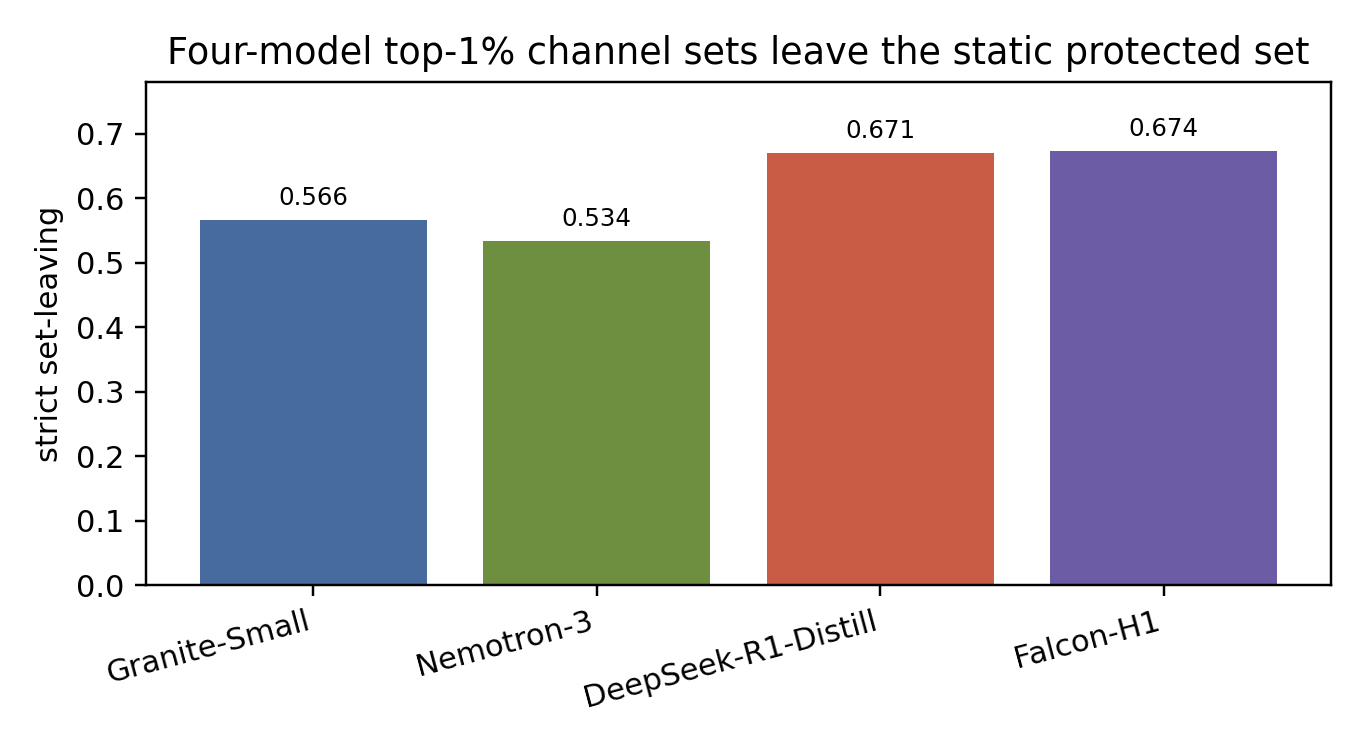
\includegraphics{figures/top1_set_leaving.png}
\caption{Top-1 set leaving}
\end{figure}

Figure 1: Four-model top-1\% set-leaving. More than half of later
high-risk channels leave the static protected set in every reported
headline model. This is cached measurement evidence, not a
positive-method claim.

\hypertarget{measurement-setup-and-error-model}{%
\subsection{2. Measurement Setup And Error
Model}\label{measurement-setup-and-error-model}}

For a top-k channel threshold, define the protected set at one trace
segment and ask how many later high-risk channels are outside that set.
This is strict set-leaving. A value near zero would support static
protection; a value above one half means the static set misses a large
portion of later high-risk channels.

Within-set shuffling is measured separately: among channels that remain
inside the protected set, their relative rank can still change. This
affects allocation inside a fixed protected set but cannot recover
channels that leave the set entirely.

The downstream relevance of set-leaving follows from a simple error
model. A channel inside the protected set incurs protected per-channel
error \(\varepsilon_p\); a high-risk channel that has left it incurs
unprotected error \(\varepsilon_q \gg \varepsilon_p\). Let
\(L=L(t_0,t)\) be the fraction of later high-risk channels outside the
set chosen at \(t_0\). Then

\[E[\mathrm{err}(t)] \approx K\{\varepsilon_p(1-L) + \varepsilon_q L\}.\]

which is increasing in \(L\). Set-leaving is therefore not merely a
membership statistic: under this model the measured \(L\) of
\(0.53\)--\(0.67\) places a large fraction of later high-risk channels
at the unprotected error rate. The model assumes leaving channels carry
comparable risk to those retained; we treat the per-channel error
attribution itself as the parked adaptive-method question and claim no
confirmed accuracy delta here.

The final regime checklist is summarized in the text below.

\hypertarget{results}{%
\subsection{3. Results}\label{results}}

\hypertarget{four-model-top-1-strict-set-leaving-is-large}{%
\subsubsection{3.1 Four-Model Top-1\% Strict Set-Leaving Is
Large}\label{four-model-top-1-strict-set-leaving-is-large}}

\begingroup\small
\begin{longtable}[]{@{}lrrl@{}}
\toprule
Model & Strict set-leaving & Within-set shuffling & Artifact
status\tabularnewline
\midrule
\endhead
Granite-Small & \(0.566235\) & \(0.270935\) & threshold sweep
available\tabularnewline
Nemotron-3 & \(0.533713\) & \(0.269082\) & threshold sweep
available\tabularnewline
DeepSeek-R1-Distill & \(0.670573\) & \(0.165737\) & threshold
sweep available\tabularnewline
Falcon-H1 & \(0.673611\) & \(0.097538\) & top-1 decomposition
available\tabularnewline
\bottomrule
\end{longtable}
\endgroup

The top-1\% values all exceed \(0.53\), and the largest reaches
\(0.673611\). Static protection is therefore not a sufficient
abstraction for these traces.

\hypertarget{the-result-is-stable-across-available-threshold-sweeps}{%
\subsubsection{3.2 The Result Is Stable Across Available Threshold
Sweeps}\label{the-result-is-stable-across-available-threshold-sweeps}}

\begin{figure}
\centering
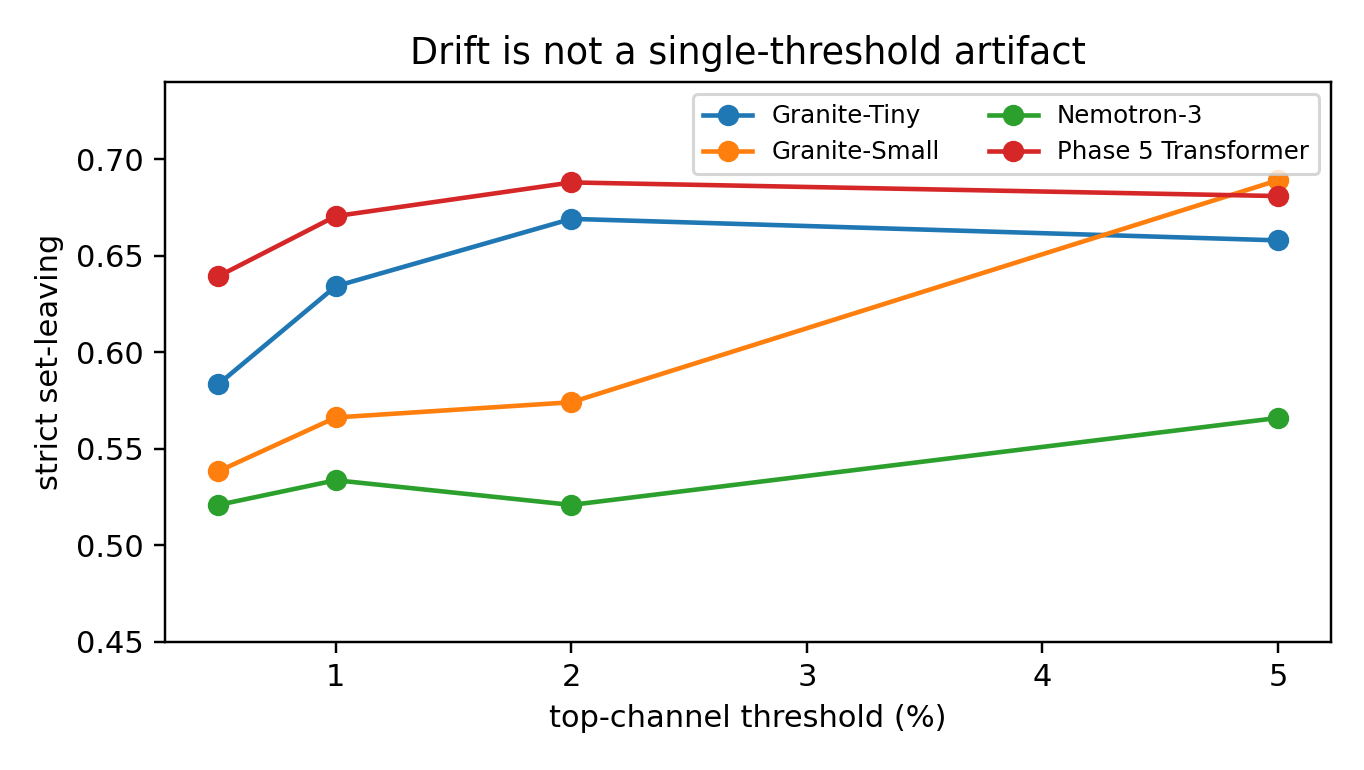
\includegraphics{figures/threshold_sensitivity.png}
\caption{Threshold sensitivity}
\end{figure}

Figure 2: Cached threshold sweep for Granite-Small, Nemotron-3, and
DeepSeek-R1-Distill. Strict set-leaving remains high across 0.5\%, 1\%,
2\%, and 5\%. Falcon-H1 is omitted here because only its top-1
decomposition artifact is available.

The threshold sweep reports all thresholds rather than selecting one
post hoc. The exact values move, but the regime does not: strict
set-leaving stays high across nearby thresholds for the models with
sweep artifacts.

\hypertarget{strict-leaving-dominates-within-set-shuffling}{%
\subsubsection{3.3 Strict Leaving Dominates Within-Set
Shuffling}\label{strict-leaving-dominates-within-set-shuffling}}

\begin{figure}
\centering
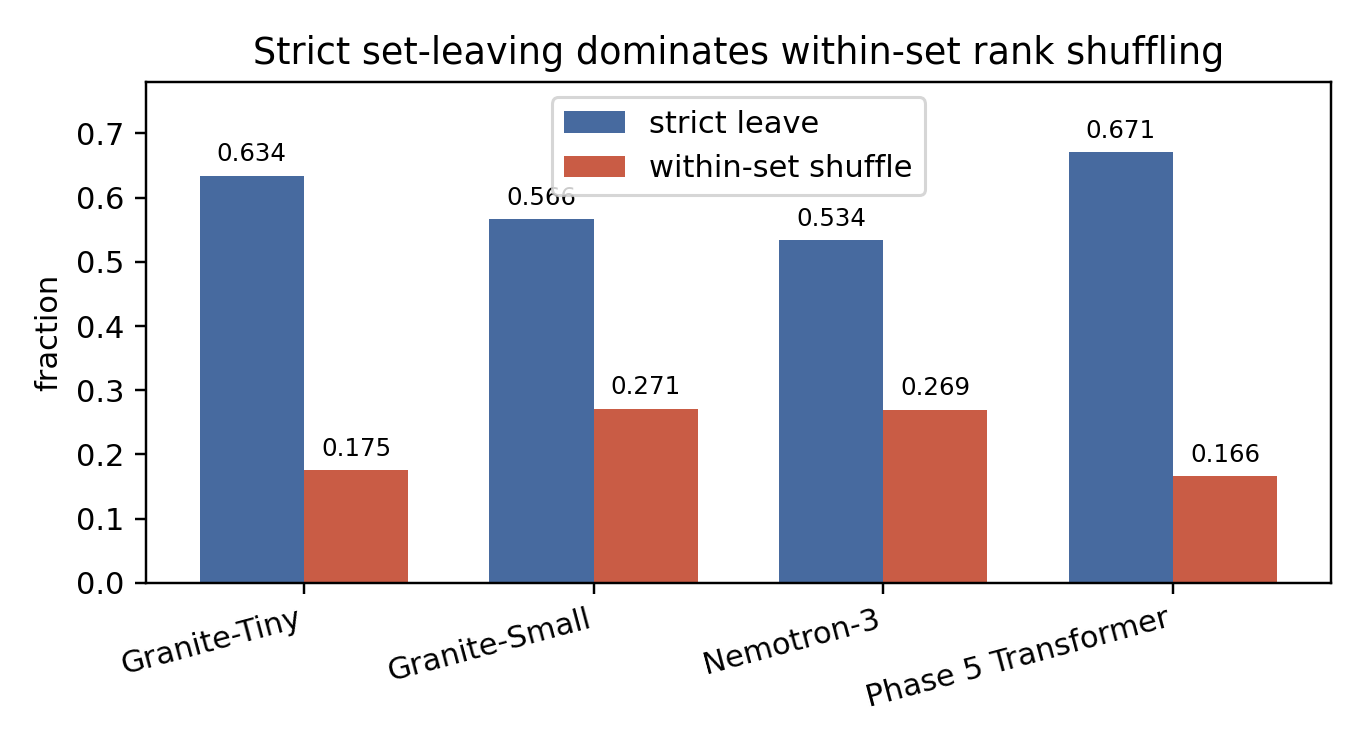
\includegraphics{figures/within_set_shuffling.png}
\caption{Within-set shuffling}
\end{figure}

Figure 3: Four-model strict set-leaving versus within-set shuffling.
Within-set shuffling exists, but strict set-leaving is the larger
effect.

Within-set shuffling at top 1\% ranges from \(0.097538\) to
\(0.270935\). That is nontrivial, but it is smaller than strict
set-leaving. The main failure mode for a static set is not only that the
protected channels change rank; many later high-risk channels are absent
from the protected set at all.

\hypertarget{why-the-adaptive-clip-candidate-is-parked-not-confirmed}{%
\subsection{4. Why the adaptive clip candidate Is Parked, Not
Confirmed}\label{why-the-adaptive-clip-candidate-is-parked-not-confirmed}}

\begin{figure}
\centering
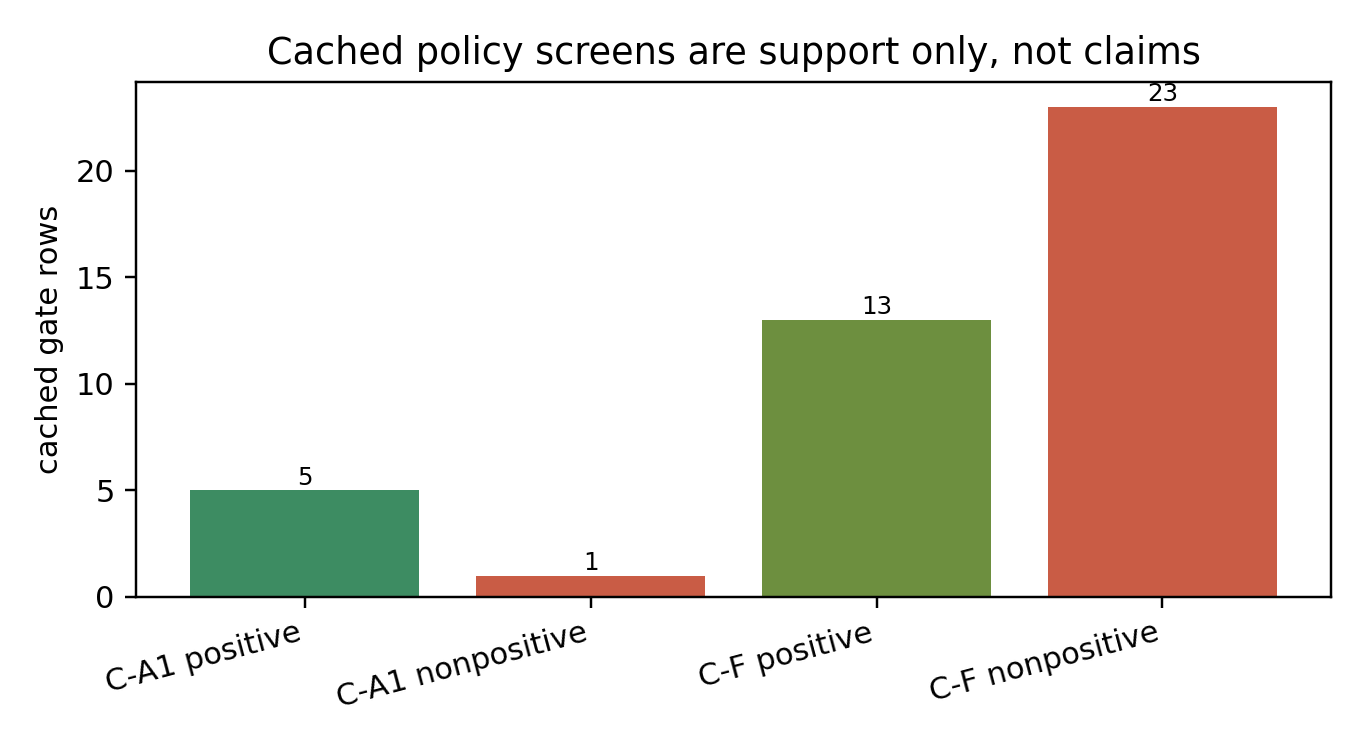
\includegraphics{figures/paroquant_vs_channelset_methods.png}
\caption{Cached policy screens}
\end{figure}

Figure 4: Cached the adaptive clip candidate and the survival-core
candidate screens are support evidence only. They are not native
same-row ParoQuant comparisons and cannot carry a positive claim.

the adaptive clip candidate remains the nearest positive-method
candidate, but it is not a paper claim. The cached screen has only
\(6\) the adaptive clip candidate gate rows, with \(5\)
positive medians and \(1\) nonpositive median. That is enough to
motivate a fresh materialization, not enough to claim a method.

\begin{figure}
\centering
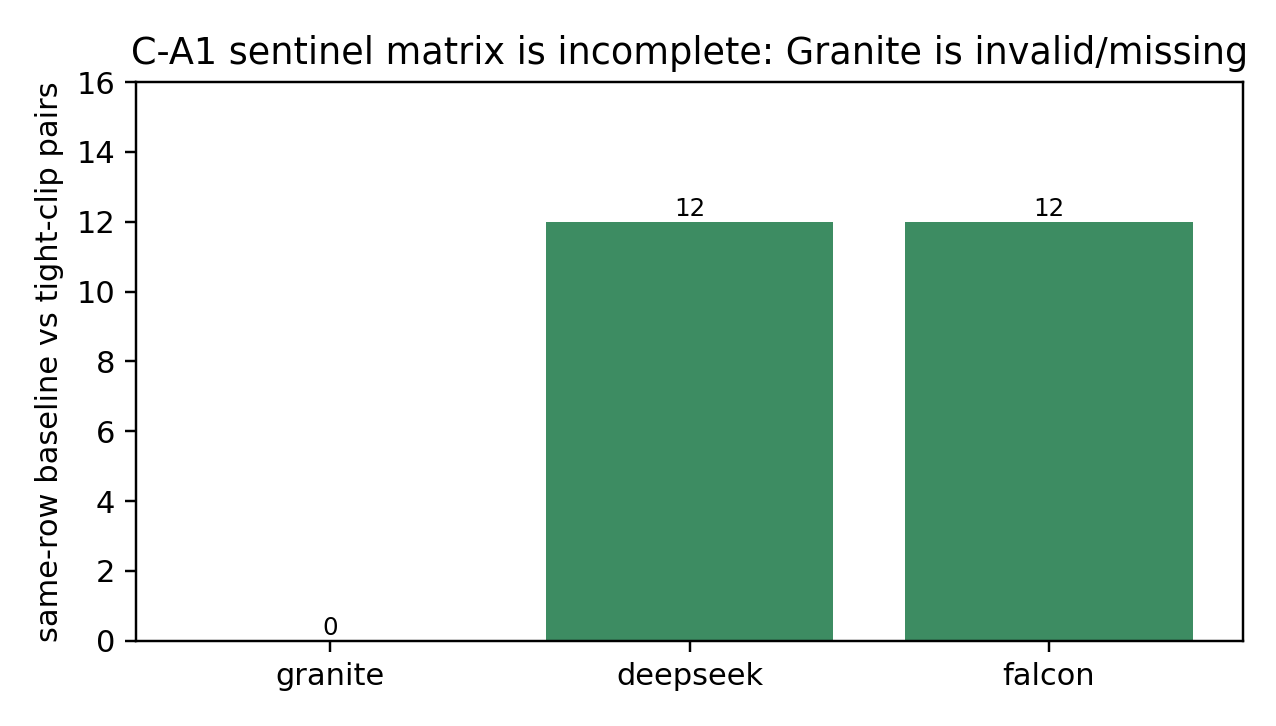
\includegraphics{figures/c_a1_sentinel_status.png}
\caption{the adaptive clip candidate sentinel status}
\end{figure}

Figure 5: The split-clean the adaptive clip candidate sentinel matrix is
incomplete. DeepSeek and Falcon have \(12\) same-row pairs, while
Granite has \(0\) valid same-row pairs in the safe manifest.

The blocker is concrete and unavoidable. A future claim needs a
Granite/DeepSeek/Falcon same-row matrix with ParoQuant baseline and
tight-clip the adaptive clip candidate outputs. The safe manifest has
DeepSeek and Falcon same-row pairs, but Granite is missing/invalid. the
adaptive clip candidate remains parked until this is rebuilt. This paper
therefore does not claim a the adaptive clip candidate win, does not
claim to beat ParoQuant, and does not claim held-out confirmation.

\hypertarget{defense-scaffold-and-schema-blockers}{%
\subsection{5. Defense Scaffold And Schema
Blockers}\label{defense-scaffold-and-schema-blockers}}

\begin{figure}
\centering
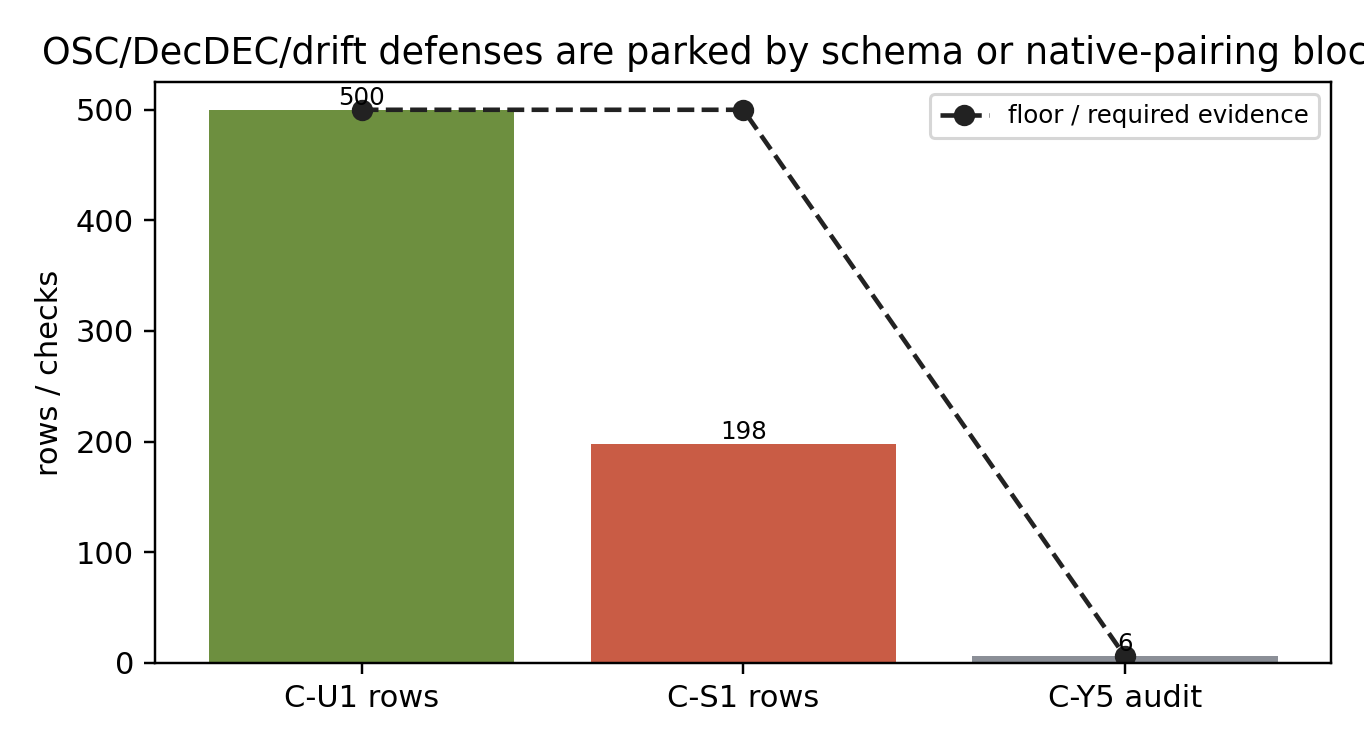
\includegraphics{figures/osc_decdec_drift_defense.png}
\caption{OSC DecDEC drift defense status}
\end{figure}

Figure 6: Defense and router ideas are a blocker map, not completed
defense proof. They are blocked by missing labels, insufficient rows, or
missing native pairing.

The defense stack is useful because it prevents overclaiming:

\begin{itemize}
\tightlist
\item
  the router audit materializes \(500\) KL trajectory rows, but
  lacks paired difficulty/policy-uplift labels.
\item
  the clean-denominator audit finds only \(198\) eligible rows
  against a \(500\) row floor. The floor is not lowered.
\item
  the defense-bundle audit has defense inputs and audit checks, but the
  three-model native the adaptive clip candidate-vs-ParoQuant packet is
  missing.
\end{itemize}

These are honest blockers, not negative proof against every future
method. They define the evidence required before a positive Channel-Set
method can be claimed.

\hypertarget{related-work-and-regime-guidance}{%
\subsection{6. Related Work And Regime
Guidance}\label{related-work-and-regime-guidance}}

Channel-Set is closest to W4A16 quantization, outlier-channel
protection, rotation-based quantization, and residual correction methods
such as ParoQuant \citep{paroquant2026}, OSC \citep{osc2026}, DecDEC
\citep{decdec2024}, ResQ \citep{resq2024}, OSCAR \citep{oscar2026}, and
OScaR \citep{oscar_kv2026}. Those systems are the correct baseline
family for any future adaptive method.

The distinguishing view here is the long-reasoning channel-set object
itself. Rather than assuming a protected channel set and measuring final
answer accuracy, this paper measures whether the protected set remains
the same object over the reasoning trace.

The regime checklist is the deliverable. A future method must measure
drift, lock ParoQuant/static/EMA baselines, preserve no-gap
denominators, require same-row native evidence, and treat the adaptive
clip candidate-like tail/CVaR policies as parked until the full matrix
exists.

\hypertarget{limitations}{%
\subsection{7. Limitations}\label{limitations}}

This is a measurement/regime paper, not a confirmed positive-method
paper. the adaptive clip candidate remains parked. The paper does not
claim to beat ParoQuant, does not claim a native GPU result, and does
not claim held-out method confirmation.

The measurements are cached decomposition evidence. They are strong
enough to establish the static-set drift regime, but a method claim
needs fresh split-clean native paired rows, model/policy hashes, no-gap
denominators, and write-once per-trace evidence.

The claim is also not that static channel sets are always wrong. It is
that, in these long-reasoning packets, strict set-leaving is large
enough that static protection alone is a weak abstraction.

\hypertarget{conclusion}{%
\subsection{8. Conclusion}\label{conclusion}}

Channel-Set contributes a scoped but useful result: long-reasoning
outlier channel sets drift. At top 1\%, more than half of later
high-risk channels leave the static protected set in every reported
headline model. That turns static W4A16 protection from a stable object
into a fragile assumption. A positive method may still emerge from the
adaptive clip candidate or related adaptive policies, but only after
fresh split-clean native paired materialization and the full
ParoQuant/audit gate.


\bibliographystyle{../colm2026_conference}
\bibliography{../references}

\end{document}
